\documentclass[showpacs, oneside, onecolumn, prl, amsmath, amssymb, nofootinbib, superscriptaddress, notitlepage]{revtex4-1}


\usepackage{cases}
\usepackage{amsmath}
\usepackage{amssymb}
\usepackage{amsfonts}
\usepackage{amssymb}
\usepackage{dcolumn}
\usepackage{bm}
\usepackage{bbm}
\usepackage{graphicx}
\usepackage{xcolor}
\usepackage{array}
\usepackage{subfigure}
\usepackage{hyperref}
\usepackage{multirow}
\usepackage{ulem}

%%%%%%%%%%%%%%%%%%%%%%%%%%%%%%%%%%%%%%%%%%%%%%%%%%%%%%%%%%%%%%%%%%%%%%%%%%%%%%%%%%%
\newcommand{\bra}[1]{\langle #1\vert}
\newcommand{\ket}[1]{\vert #1\rangle}
\newcommand{\nn}{\nonumber \\}
\newcommand{\lag}{\langle}
\newcommand{\rag}{\rangle}
\newcommand{\cN}{{\cal N}}
\newcommand{\cA}{{\cal A}}
\newcommand{\gsim}{\mathrel{\hbox{\rlap{\lower.55ex \hbox {$\sim$}}
                   \kern-.3em \raise.4ex \hbox{$>$}}}}
\newcommand{\lsim}{\mathrel{\hbox{\rlap{\lower.55ex \hbox {$\sim$}}
                   \kern-.3em \raise.4ex \hbox{$<$}}}}

\newcommand\be{\begin{equation}}
\newcommand\ba{\begin{align}}
\newcommand\bas{\begin{align*}}
\newcommand\bt{\begin{table}}
\newcommand\bts{\begin{table*}}
\newcommand\bfig{\begin{figure}}
\newcommand\bfs{\begin{figure*}}
\newcommand\ee{\end{equation}}
\newcommand\ea{\end{align}}
\newcommand\et{\end{table}}
\newcommand\ets{\end{table*}}
\newcommand\efig{\end{figure}}
\newcommand\efs{\end{figure*}}
\newcommand\RA{$\ \ \Rightarrow\ \ $}
\newcommand\MC{\mathcal}
\newcommand\MBF{\mathbf}
\newcommand\MBB{\mathbb}

\newcommand\blue{\textcolor{blue}}
\newcommand\gray{\textcolor{gray}}
\newcommand\green{\textcolor{teal}}
\newcommand\red{\textcolor{red}}




\hypersetup{colorlinks=true,
            breaklinks=true,
            pdfstartview=Fit,
            linkcolor=blue,
            citecolor=green,
            urlcolor=blue}

\bibliographystyle{apsrev4-1}




%%%%%%%%%%%%%%%%%%%%%%%%%%%%%%%%%%%%%%%%%%%%%%%%%%%%%%%%%%%%%%%%%%%%%%%%%%%%%%%%%%%
\begin{document}
	
\title{Problem Set 7 for PDEs}

\author{JIAO Hao}

\maketitle

~~~~

%%%%%%%%%%%%%%%%%%%%%%%%%%%%%%%%%%%%%%%%%%%%%%%%%%%%%%%%%%%%%%%%%%%%%%%%%%%%%%%%%%%
\section{Problem 1}

Set $f(x,t)=\xi^t\exp(ikx)$.

\bas
&\frac{\partial f}{\partial t}+v\frac{\partial f}{\partial x}=0\\
\Rightarrow\ \ &v=-\frac{\partial f/\partial t}{\partial f/\partial x}=-\frac{\ln\xi}{ik}=i\ln(\xi)/k
\end{align*}

%\bas
%f(t,x+dx)-f(t,x-dt)&=\xi^t(\exp[ik(x+dx)]-\exp[ik(x-dx)])\\
%&=\xi^t\exp(ikx)(e^{ikdx}-e^{-ikdx})
%\end{align*}

\bas
f(t+dt,x)&=\xi^{t+dt}\exp(ikx)=\xi^t\exp(ikx)\cdot e^{\ln(\xi)dt}\\
&=f(t-dt,x)-\frac{v\,dt}{dx}[f(t,x+dx)-f(t,x-dx)]\\
&=\xi^{t-dt}\exp(ikx)-\frac{v\,dt}{dx}[\xi^t\exp[ik(x+dx)]-\xi^t\exp[ik(x-dx)]]\\
&=\xi^t\exp(ikx)[\xi^{-dt}-\frac{v\,dt}{dx}(e^{ikdx}-e^{-ikdx})]
\end{align*}

\bas
&\Rightarrow\ \ \xi^{dt}=\xi^{-dt}-\frac{v\,dt}{dx}(e^{ikdx}-e^{-ikdx})\\
&\Rightarrow\ \ (\xi^{dt})^2+\alpha(e^{ikdx}-e^{-ikdx})\xi^{dt}-1=0\\
&\Rightarrow\ \ (\xi^{dt})^2+2i\alpha\sin(kdx)\xi^{dt}-1=0
\end{align*}
where $\frac{v\,dt}{dx}=\alpha$

\bas
&\Rightarrow\ \ \xi^{dt}=-i\alpha\sin(kdx)\pm\sqrt{1-(\alpha\sin(kdx))^2}
\end{align*}

%\RA $\xi^{dt}=e^{\ln\xi\,dt}=e^{-ik\alpha dx}$
%\bas
%&\xi^{dt}-[\xi^{-dt}-\frac{v\,dt}{dx}(e^{ikdx}-e^{-ikdx})]\\
%=\,&\xi^{dt}-\xi^{-dt}+\frac{v\,dt}{dx}(e^{ikdx}-e^{-ikdx})\\
%=\,&e^{-ik\alpha dx}-e^{ik\alpha dx}+\alpha(e^{ikdx}-e^{-ikdx})\\
%=\,&-2i\sin(\alpha kdx)+2i\alpha\sin(kdx)
%\end{align*}

If the CFL condition is satisfied $\alpha<1$ \RA $1-(\alpha\sin(kdx))^2>0$ so the second term is the real part \RA
\bas
|\xi^{dt}|^2=1-(\alpha\sin(kdx))^2+(\alpha\sin(kdx))^2\equiv1
\end{align*}

So the leapfrog scheme preserves energy

~~~~

~~~~

~~~~

%%%%%%%%%%%%%%%%%%%%%%%%%%%%%%%%%%%%%%%%%%%%%%%%%%%%%%%%%%%%%%%%%%%%%%%%%%%%%%%%%%%
\section{Problem 2}

%%%%%%%%%%%%%%%%%%%%%%%%%%%%%%%%%%%%%%%%
\subsection{part a. A point charge}


%------
\bfig
	\centering
	\subfigure
	{\begin{minipage}[b]{1\textwidth}
	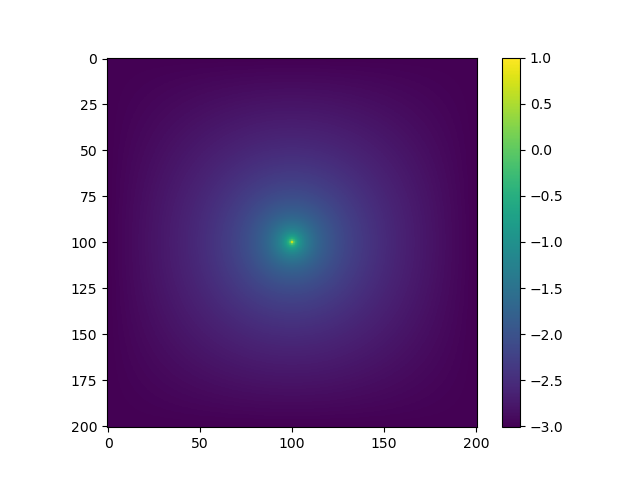
\includegraphics[scale=0.9]{7-2-1.png}
	\end{minipage}}
	\subfigure
	{\begin{minipage}[b]{1\textwidth}
	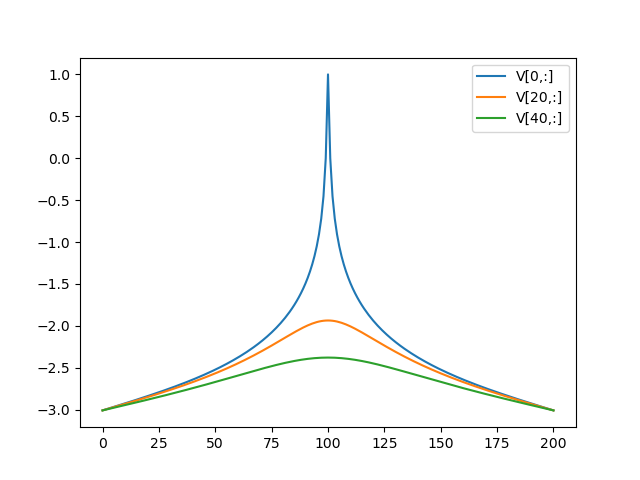
\includegraphics[scale=0.9]{7-2-1-2.png}
	\end{minipage}}
	\caption{Potential from a point charge. The top penal is the 2D potential, and the bottom penal shows several section of the potential.}
	\label{7-2-1}
\efig


I set $\rho[0,0]=1$, and all others are 0. and the potential also defined at the center($[100,100]$). To let $V[0,0]=1$, I set $V=V-V[n//2,n//2]+1$ at the end. The potential is shown in fig.\ref{7-2-1}

The potential of several points:

\gray{$V[0,0]=1$}

\gray{$V[1,0]=4.4408e-15\sim0$}

\gray{$V[2,0]=-0.45352$}

\gray{$V[5,0]=-1.0516$}


~~~~

%------
\bfig
	\centering
	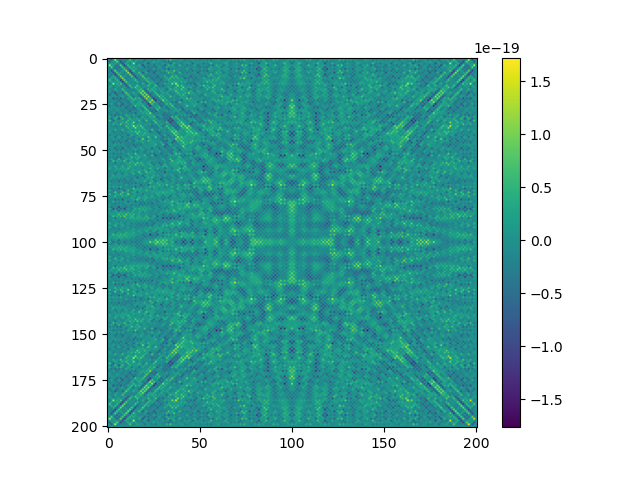
\includegraphics[scale=0.8]{7-2-1 rk.png}
	\caption{The residue rk at the end.}
	\label{7-2-1 rk}
\efig

Here is the residue and the final rk is shown in fig.\ref{7-2-1 rk}

\gray{residue of 0 is 0.25}

\gray{residue of 100 is 0.003142653852739444}

\gray{residue of 200 is 1.724840022148694e-05}

\gray{residue of 300 is 2.46762839628658e-11}

\gray{residue of 400 is 5.204556450512147e-19}

\gray{residue of 500 is 2.9413100149531863e-30}

\gray{residue of 600 is 5.065917816941024e-35}

~~~~

~~~~

%%%%%%%%%%%%%%%%%%%%%%%%%%%%%%%%%%%%%%%%
\subsection{part b. Charge density}

%------
\bfig
	\centering
	\subfigure
	{\begin{minipage}[b]{1\textwidth}
	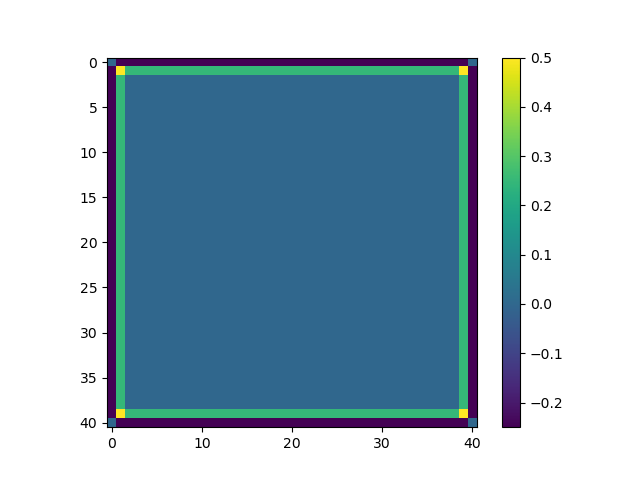
\includegraphics[scale=0.9]{7-2-2-1.png}
	\end{minipage}}
	\subfigure
	{\begin{minipage}[b]{1\textwidth}
	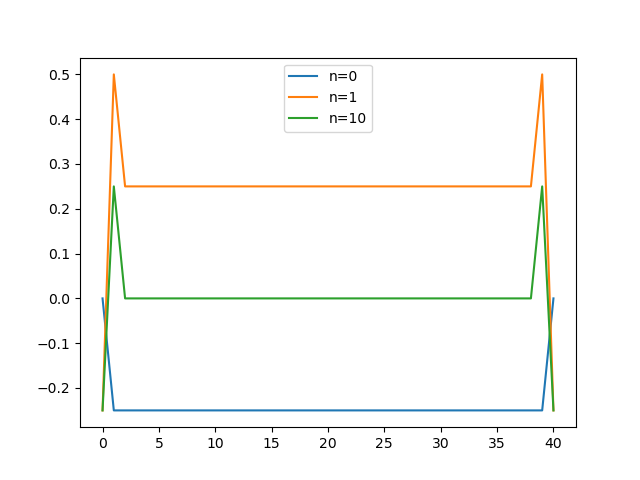
\includegraphics[scale=0.9]{7-2-2-2.png}
	\end{minipage}}
	\caption{Charge density of a flat potential. The top penal is the 2D charge density, and the bottom penal shows several section of the charge density.}
	\label{7-2-2}
\efig

I set the potential equal to 1 except for the boundary ($=0$), and the charge density is show in fig.\ref{7-2-2}.


~~~~

~~~~

%%%%%%%%%%%%%%%%%%%%%%%%%%%%%%%%%%%%%%%%
\subsection{part c. Potential of the above charge}

%------
\bfig
	\centering
	\subfigure
	{\begin{minipage}[b]{1\textwidth}
	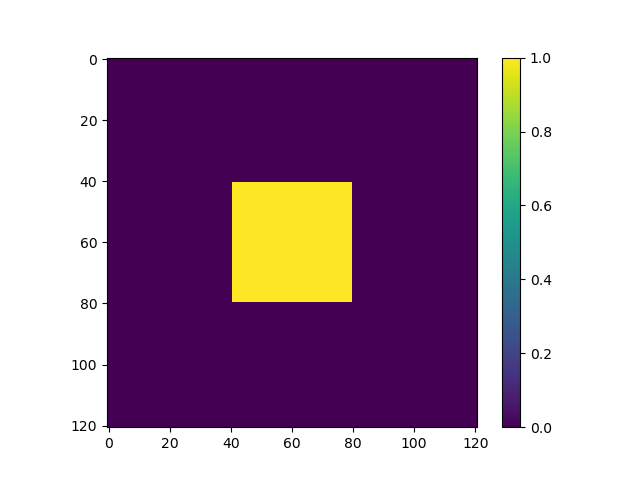
\includegraphics[scale=0.9]{7-2-3-3.png}
	\end{minipage}}
	\subfigure
	{\begin{minipage}[b]{1\textwidth}
	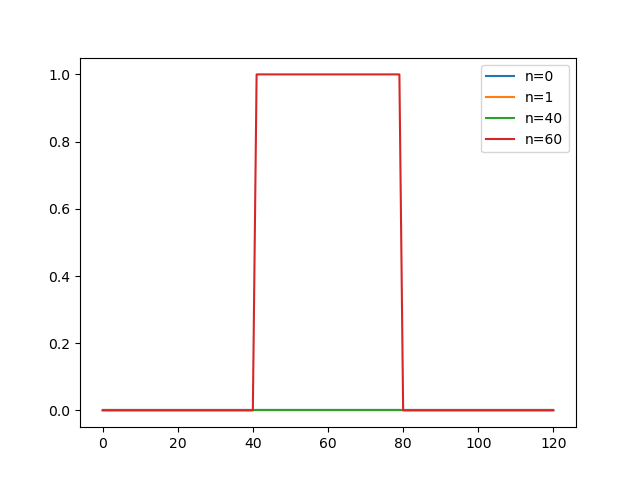
\includegraphics[scale=0.9]{7-2-3-4.png}
	\end{minipage}}
	\caption{Charge density of a flat potential. The top penal is the 2D charge density, and the bottom penal shows several section of the charge density.}
	\label{7-2-2}
\efig

Using the charge density above (in a box with width n=41) and get the potential. We can see that it is really a square potential at the box.









\end{document}